 
%---------------------------------------------------------------------------
% Content of Chapter 6 - Implementation
%
%---------------------------------------------------------------------------


\chapter{Implementation details}
\label{cha:implementation}

Within this chapter dear may find rough implementation details of SemSimMon application. I don't intent to cover
source code in detail, instead I'd like to describe most important interfaces, technologies  that were
employed during implementation and will try to bring some light on source code structure. The main goal I want to
achieve with it is to lower the learning curve, needed to continue working on the project by other developers.

Each an every component of SemSimMon system was implemented using Java programming language. Decision to use this
particular technology is quite obvious, after even rough analysis of requirements that system must met. Java is
actually the most mature, cross platform programming language, so during development there is no need to worry about
platform specific issues, as it's part of Java Virtual Machine vendor responsibility. Additionally, as one of major
requirements is to be able to monitor processes running on JVM, using JMX protocol. The second communication
requirement - interactions with OMIS compliant tools, can be easily achieved using Java bindings for OCM-G
platform\footnote{\url{http://grid.cyfronet.pl/ocmg/japi.html}}.  

Although building mechanism isn't directly part of implementation, understanding this process is crucial for someone
who would like to work with project. SemSimMon uses Apache Maven\footnote{\url{http://maven.apache.org/}} as build
manager. Maven recently became the de facto standard in building Java based projects. Features like dependencies
management, build configuration instead of scripting actions needed to build project and extensive usage of plug-in
architecture. Project configuration uses maven's aggregation mechanism to ease dependencies and configuration
management. Project structure contains following maven modules:

 
\begin{itemize}
 \item pl.edu.agh.semsimmon:semsimmon - root module
 \item pl.edu.agh.semsimmon:gui - GUI component
 \item pl.edu.agh.semsimmon:mon-hub - Monitoring Hub component
 \item pl.edu.agh.semsimmon:mon-hub-app - Monitoring Hub Application component 
 \item pl.edu.agh.semsimmon:commons - component containing Transfer Objects and interfaces shared among all other
components
 \item pl.edu.agh.semsimmon:knowledge - Knowledge component
 \item pl.edu.agh.semsimmon:transports - parent module for all transport components
 \item pl.edu.agh.semsimmon.transports:jmx - JMX Transport component
 \item pl.edu.agh.semsimmon.transports:ocmg - OCM-G Transport component
\end{itemize}


Using Java as main implementation technology has another significant implication - wide usage and uncounted amount of
open source libraries that can shorten development time.



\section{Common frameworks}

There are two areas of implementation that are shared among all components, namely logging and testing. As a logging
framework, SemSimMon uses combined slf4j\footnote{\url{http://www.slf4j.org}} and
log4j\footnote{\url{http://logging.apache.org/log4j}} libraries. Apache Log4j is probably most widely used logging
framework for Java and is known for it's low performance impact and extensive configuration options. slf4j stands for
Simple Logging Facade for Java, it's main purpose is to simplify logging interface even more, and decouple code from
actual logging framework. This is quite important, as logging invocations tends to spread over code, which makes any
change in logging facility quite a challenging task. With slf4j changing logging framework requires only change in
configuration code.

As a testing framework, SemSimMon uses 2 libraries: TestNG\footnote{\url{http://testng.org/doc/index.html}} and
mockito\footnote{\url{http://mockito.org/}}. TestNG provides test runners and means to implement test cases. On the
other hand, mockito is excellent library for implementing unit tests - it provides facility for creating easy to use
mock objects, which are essential in Test Driven Development.

 
%---------------------------------------------------------------------------
% Gui component.
%
%---------------------------------------------------------------------------


\section{GUI component}
\label{sec:arch_gui}

Graphical user interfaces are most commonly used form of interaction with user in modern computing. Designing decent
user interface is especially important due to aim of this work - creation of application allowing measuring and
visualization of monitored processes. Although GUI component has rather limited role of giving user control over
application and allow to view results of the work it's in fact most complex component. Additionally any shortcoming in
GUI is relatively difficult to be hidden by user, and that makes UI/UX (User Interface/User Experience) engineering so
important.

During designing user interface I've been trying to follow few general principles. First of all, I wanted used
interface to be as transparent as possible. Users should focus on their tasks instead of application. Because of that,
interface shouldn't be bloated with unnecessary options and steps that users need to achieve their goals should be as
short as possible. Next equally important interface item are visualizations. Because visualizations are most important
functionality of application, they need special concern. User should be able to view charts with results with out
any interruptions blocking or any other UI components that might be disturbing. What is also important, GUI must be
coherent to free user from chaos of being spread across multiple windows, desktops. 

From business logic point of view, GUI component will extensively use MVC design pattern\cite{gamma1995}. Each form,
window or more complex section need to have it's own View, responsible for presentation, Controller that collects
user's events and updates view on user's actions or system events. Application will have shared model, which will be
access point for underlaying components.
 


\subsection{Interface Mockups}

In this section, will try to describe mockups of most important views. The first mockup depicted in
Figure~\ref{fig:mock_main} shows main application view. Left edge of application window contains vertical tab pane
controller that will allow user to easily switch views covering 3 most important application contexts - resources,
measurements and visualizations. Another benefit of such a approach is that application has loads of space for what
user actually needs. The second most important component of main view is menu bar placed on top. It allows user
to perform bulk operations (e.g. pause all measurements) regardless of view he or she is currently. 

All subsequent mockups covers context specific views that will be rendered in main view's central pane.



\begin{figure}[ht]
  \centering
  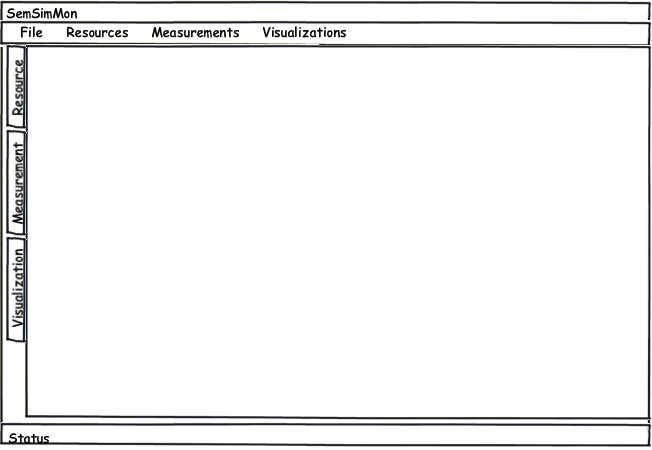
\includegraphics[width=0.7\textwidth]{mock_main}
  \caption{GUI application main view mockup}
  \label{fig:mock_main}
\end{figure}

When users starts to work with application He or She must add resources to be measured first. That's why resources view
is first, initial section shown to the user directly after page startup. Mockup of resources can bee seen in
Figure~\ref{fig:mock_resources}. The view is divided into 2 high level logical parts - the left pane covers global
resources context - users can browse measurement tree as well as add new resources into it. The right pane is specific
to resource selected by user and contains accordion with two sections. The upper one shows resource's static
attributes. The one below allow user to see snapshot of resource's dynamic state and check all of it's capabilities at
given point of time. To refresh those values, Refresh button was provided. Additionally, below accordion there are
several buttons allowing performing actions on given selected resource.

\begin{figure}[ht]
  \centering
  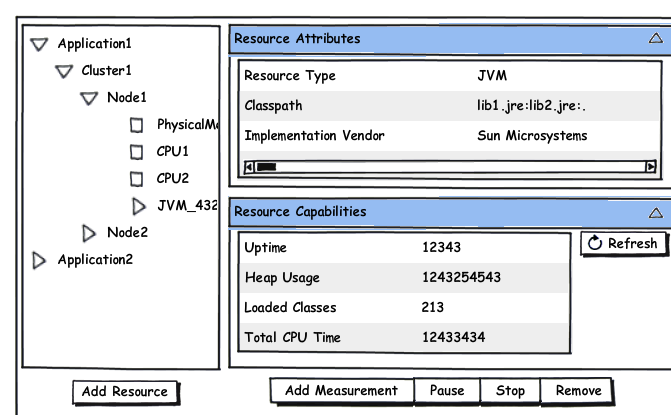
\includegraphics[width=0.7\textwidth]{mock_resources}
  \caption{GUI application resources pane}
  \label{fig:mock_resources}
\end{figure}

Next figure, Figure~\ref{fig:mock_measurements} covers measurements context of application. All measurements created
are listed on left side of this view. After selecting one accordion on right side shows details of selected
measurement. The upper section contain table with general informations. The lower one shows all measurement values
since the beginning. Additionally in this section user may copy the results into CSV format which can be easily
imported to spreadsheet application for further analysis. Using controls under measurements list, user can
pause, resume or remove measurement.

\begin{figure}[ht]
  \centering
  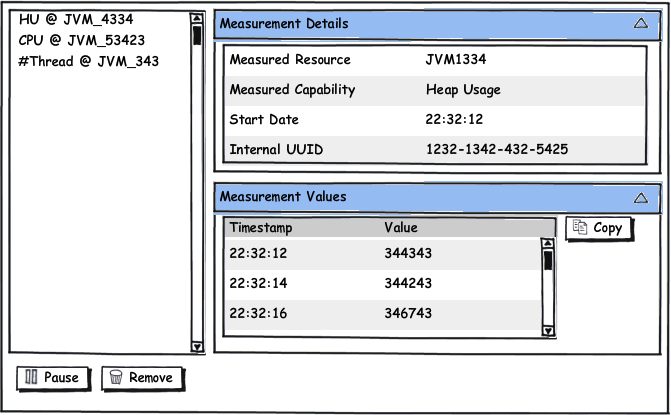
\includegraphics[width=0.7\textwidth]{mock_measurements}
  \caption{GUI application measurements pane}
  \label{fig:mock_measurements}
\end{figure}



\begin{figure}[ht]
  \centering
  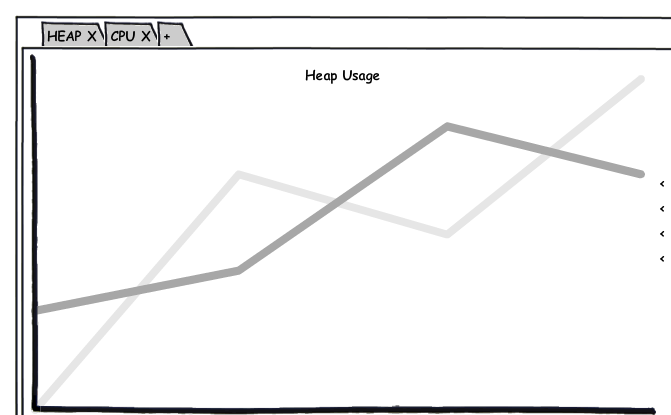
\includegraphics[width=0.7\textwidth]{mock_vis_clean}
  \caption{GUI application visualizations pane, clean view}
  \label{fig:mock_vis_clean}
\end{figure}

Appropriate visualizations display is probably most difficult for user experience engineering. During designing this UI
component I was inspiring myself from modest web browsers. The effects can be seen in Figure~\ref{fig:mock_vis_clean} -
in proposed solution every visualization is being rendered on separate, horizontal tab. To add new visualization, user
should just click last tab with appropriate icon. To remove visualization - user simply clicks cross icon on
visualization tab - just as He or She would close tab in browser. This gives visualization chart as much place as
application can give, and still allows user to easily control creation and disposal of visualization.

The biggest problem with such a approach is where to place controls of visualization. User must be able to choose which
measurements should be included in given visualization, as well as type of chart or other parameters. To address this
need, management pane was designed. It's hidden by default and is being displayed to the user, on mouse over right
edge of chart, marked with '<' signs. Layout of this pane is depicted in Figure~\ref{fig:mock_vis_options}. This
options pane contains form, divided into severals sections:

\begin{itemize}
 \item Visualization Options - user can here configure label of whole visualization, the one on tab pane
 \item Chart Options - allows setting chart's title (rendered on chart's graphics) and choose the chart type. User will
be able to use line (XY scatter), pie, bar and  spider web chart types.
 \item Measurements - gives control over which measurements should be included in given visualization. To add
measurement into visualization, user should click Add button and from displayed dialog choose which measurements should
be included. System doesn't give any constraints on measurements to be chosen, so it's up to the user to prepare
meaningful visualization. User will be able to remove given measurement from chart, by simply selecting it from list
and clicking Remove button.
 \item Actions - allows user to pause, resume visualization. Additionally user can copy to clipboard image containing
snapshot of visualization's chart.
\end{itemize}


\begin{figure}[ht]
  \centering
  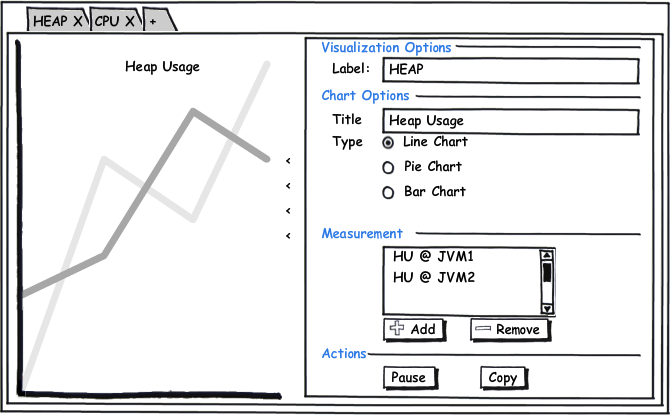
\includegraphics[width=0.7\textwidth]{mock_vis_options}
  \caption{GUI application visualizations pane, view with options pane}
  \label{fig:mock_vis_options}
\end{figure}



\subsection{Architecture}
%%-------------------------------------------------------------------------------------------
% Description of monitoring hub and monitoring hub application implementation 
%-------------------------------------------------------------------------------------------


\section{Monitoring Hub Implementation}

\section{Monitoring Hub Application Implementation}
%---------------------------------------------------------------------------
% Knowledge copmonent.
%
%---------------------------------------------------------------------------


\section{Knowledge component}
\label{sec:arch_knowledge}
 

Knowledge component is responsible for realization of semantic approach to proposed system. Although end-user can
barely notice its existence, it is crucial to allow high scalability and ease of use. Ontologies provided by
system gives generic measurement semantic. Such a approach allows user to get to know system only once and work using
it with many different types of hardware, protocols or more general - with any type of measured items that can be
mapped into generic components introduced by ontologies. Additionally it allows to work with all those different items
simultaneously, thus it makes possible monitoring application that are written using different technologies
and that are cooperating with each other.

\subsection{Default ontologies}

All system functionalities are built around two main ontologies - first one grouping resources, and the second, covering
resource capabilities. Main principle, I have been trying to follow, while designing them was to maximize wideness of
applications that can be monitored using SemSimMon system. User of application should be able to monitor wide range of
applications - from those running single process on one computing machine, up to highly distributed, grid-based ones.

To be able to describe proposed ontologies in more detail, two root concepts must be explained: concept of the
resource and the capability. Every other entity used in application is subclass of one of above. The resource
class wraps all components, either physical of virtual that are being used by user of application to
perform requested computations. Resource can be physical device that takes part in computation (hardware
resources), or any software component that can be either dependency (library) or is created by user (program, library).
On the other hand, the capability concept is used to generalize all measurable features of each resource. Capabilities
exists only in context of resources that contains them. Each resource may have multiple capabilities and given
capability may exist with multiple resources.

Above ontologies are being described using diagrams containing two types of relationships: is-a, and has-a. Is-a, is
formalized as rdfs:subClassOf and states that all the instances of one class are instances of
another\cite{rdfRef:2004}. Has-a relationship is used only to describe resources. It's main purpose is to show
composition arrangement, to ease understanding which resources are used by given parent resource to operate (e.g.
virtual machine uses class loader, garbage collector; computing node is built from one or more CPU, storage device,
network device and so on).

In following diagrams, entities are drawn as filled ellipse with entity name inside. The graphical representation of
is-a relationship between two entities is a hollow triangle shape on the supertype end of line that connects it to one
or more subtypes. To represent has-a relation, line with an arrowhead indicating entity owned by owner is used. This
notation is inspired by UML use case diagrams.

\pagebreak

\subsection{Resources ontology}
\label{subsec:arch_knowledge_resources}

Due to resources ontology complexity, diagrams containing both is-a and has-a relationships have been split into 3
parts: the one containing most general classes (application, node, cluster), second one for hardware resources
and software resources diagram.

\begin{figure}[ht]
  \centering
  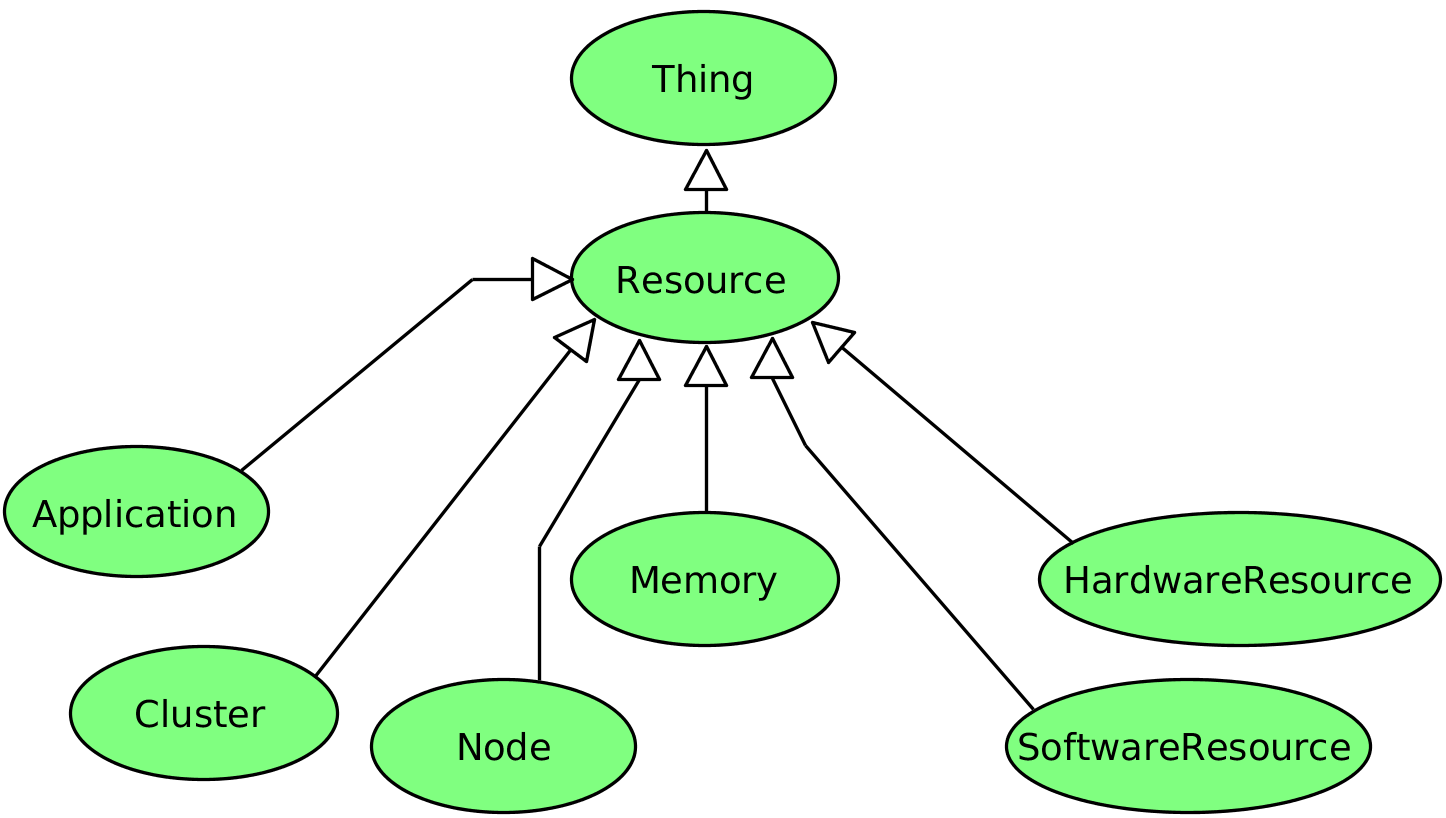
\includegraphics[width=0.6\textwidth]{onto_resources_admin}
  \caption{Diagram of is-a (rdfs:subClassOf) relationship between most general resource concepts}
  \label{fig:onto_resources_admin}
\end{figure}



Figure~\ref{fig:onto_resources_admin} depicts is-a relationship between general SemSimMon concepts. The root class of
every entity in OWL compliant ontologies is owl:Thing, as specified in OWL language reference\cite{owlRef:2004}. To
cover all possible resources - generic Resource class was introduced. It acts as a root concept for all other resources
and the only one direct subclass of owl:Thing. Resource has 6 direct subtypes: Application, Cluster, Node, Memory,
HardwareResource and SoftwareResource. Application and Cluster types are so called 'management' class resources - they
doesn't represent actual components, which can be used to perform computations. Instead, they can be used to aggregate
one or more elements, which allows user to building more manageable measurement structures. Application is most
important item, in context of has-a relationship, which illustrates Figure~\ref{fig:onto_resources_has_a_admin}. It
represent program created by user, which he or she wants to analyze using proposed tool. Each application, in
theoretical model may be running on multiple clusters, and multiple nodes.

Cluster refers to group of computing nodes which are connected using high efficiency network,thus in some way may be
treated as single entity. It is equivalent of site in OMIS nomenclature\cite{tl9702e}. Node can be interpreted as a
bridge between high-level resources and software, hardware resources. Generally speaking, it is smallest independent
computing unit, e.g. single PC or unit in a rack. It can be treated as administrative type of resource, as it's
not component that is used directly to aid computations, it rather aggregates such a components (all it's hardware with
operating system). But, on the other hand, node is an actual device that is used in processing. 

There exists also special class of resources - Memory. It's extracted to subclass Resource type directly, because there
exists at least two types of memory: software based (virtual memory) and hardware (physical memory) that share
common semantics.

\begin{figure}[ht]
  \centering
  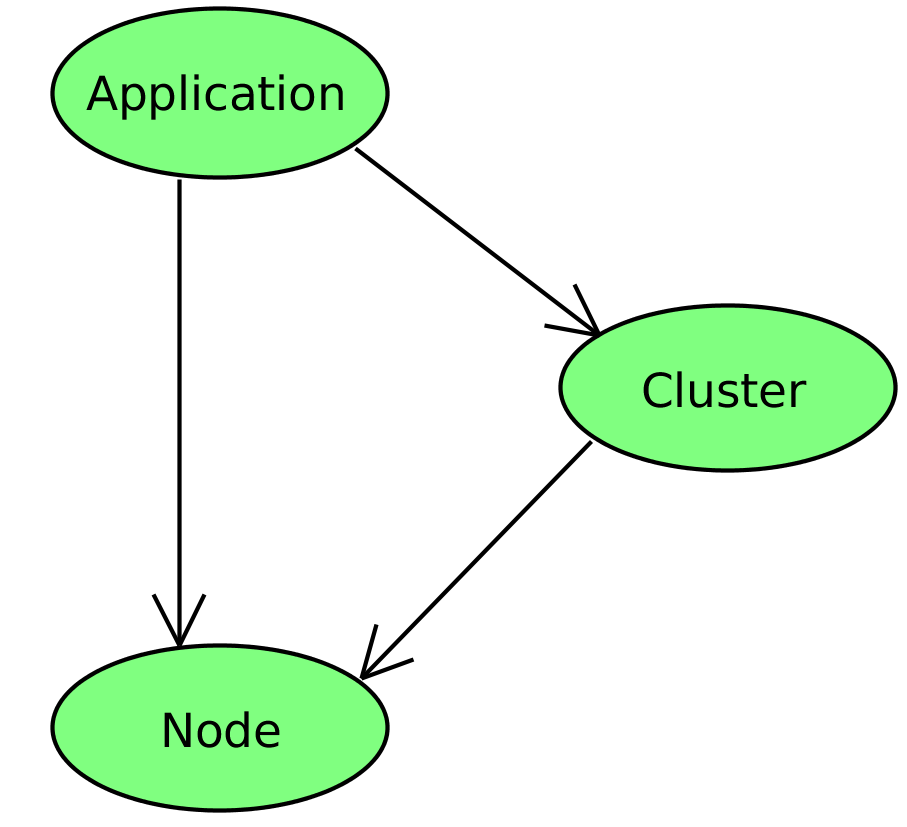
\includegraphics[width=0.3\textwidth]{onto_resources_has_a_admin}
  \caption{Diagram of has-a relationship between most general resource concepts}
  \label{fig:onto_resources_has_a_admin}
\end{figure}

\pagebreak


\begin{figure}[ht]
  \centering
  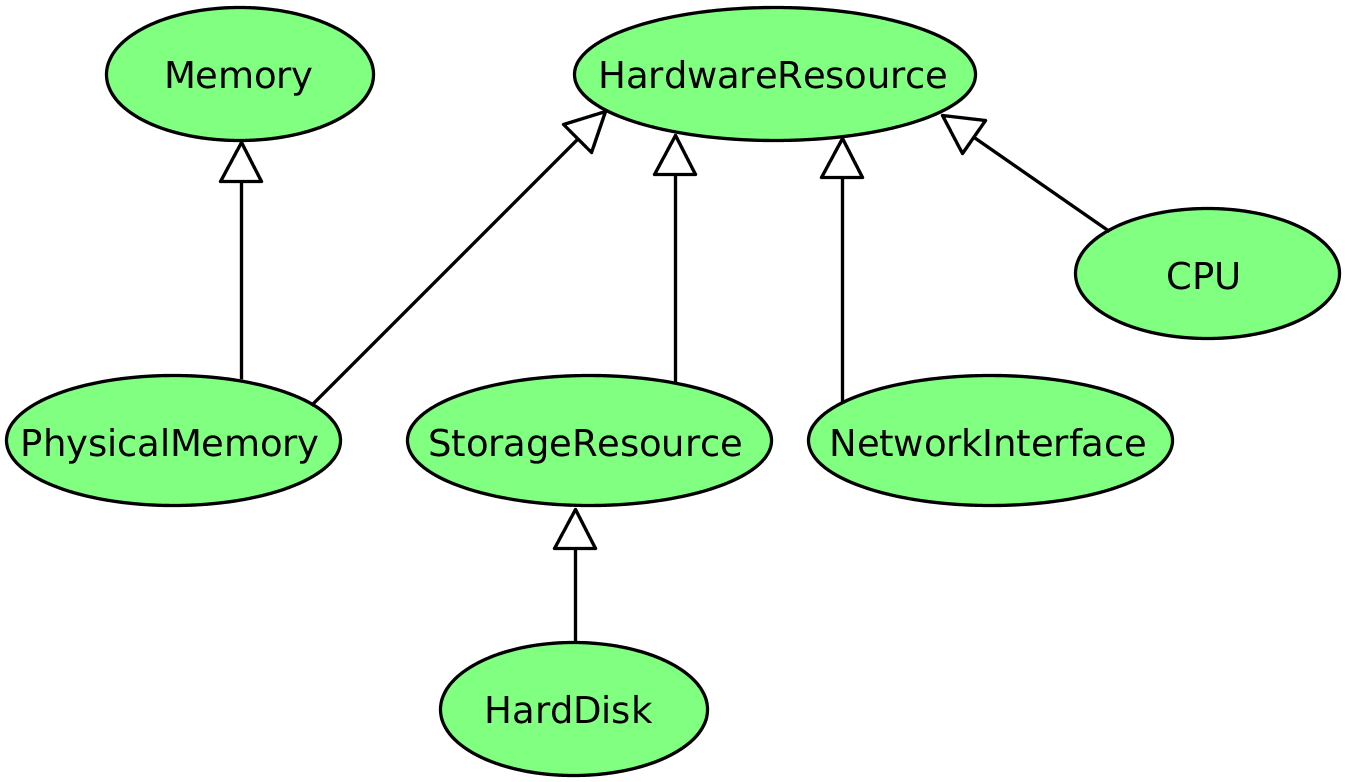
\includegraphics[width=0.6\textwidth]{onto_resources_hardware}
  \caption{Diagram of is-a relationship between hardware resources}
  \label{fig:onto_resources_hardware}
\end{figure}

Classes related to hardware resources, as can be seen in Figures~\ref{fig:onto_resources_hardware}
and~\ref{fig:onto_resources_has_a_hardware} were designed in a way that will allow to cover most of computer parts
available nowadays on market. Both diagrams are quite straightforward. HardwareResource has 4 direct sub-types:
PhysicalMemory, StorageResource, NetworkInterface and CPU. PhysicalMemory, is also subtype of Memory class, to share
common semantics, as was stated before. Also, StorageResource has one deriving class - HardDisk. 
Hardware resources has-a relationship diagram is even more elementary - Node may have all hardware resources, and there
are no other relations between those resources. Such a semantic allows to model any type of computing node - plain PC
with one, or more CPUs with at least one core (each core is treated as separate CPU).

\begin{figure}[ht]
  \centering
  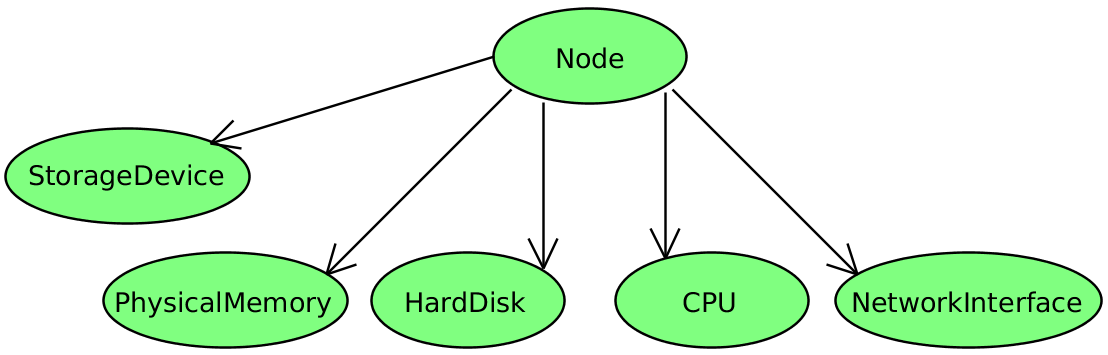
\includegraphics[width=0.7\textwidth]{onto_resources_has_a_hardware}
  \caption{Diagram of has-a relationship between hardware resources}
  \label{fig:onto_resources_has_a_hardware}
\end{figure}


\begin{figure}[ht]
  \centering
  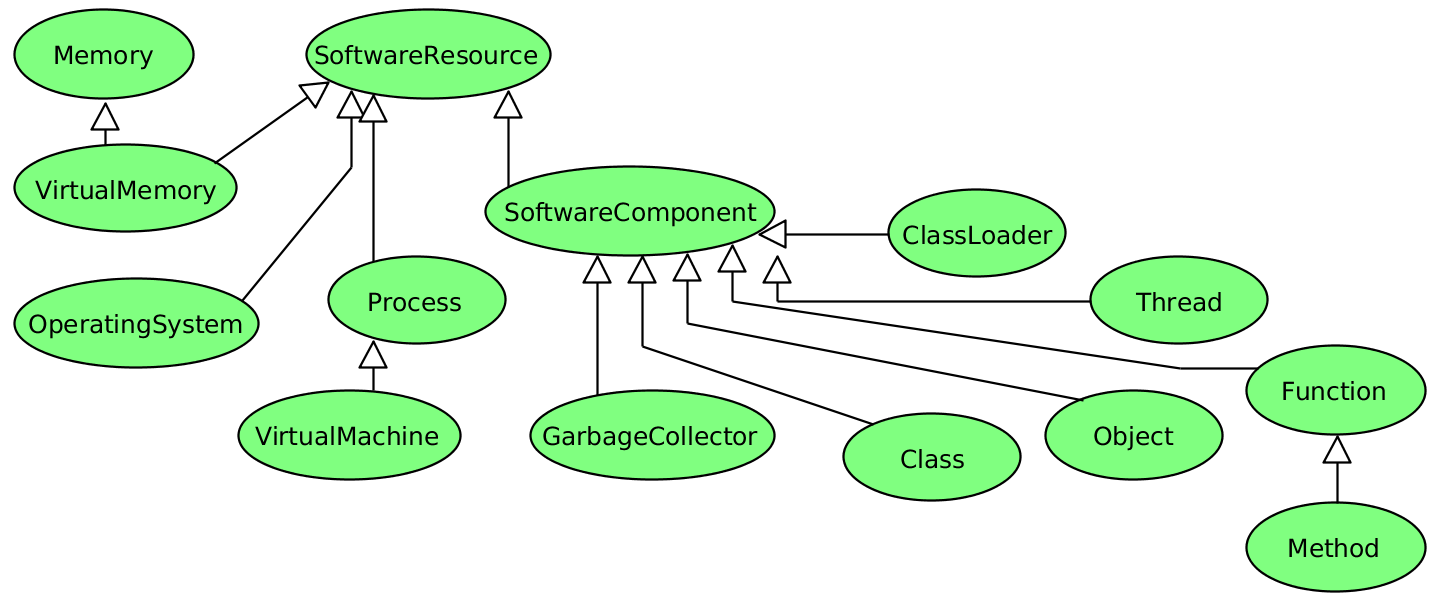
\includegraphics[width=0.9\textwidth]{onto_resources_software}
  \caption{Diagram of is-a relationship between software resources}
  \label{fig:onto_resources_software}
\end{figure}

System is aware of more software resource types then hardware ones. This implies more sophisticated relationships
between those concepts, which are depicted in Figures~\ref{fig:onto_resources_software} and
Figure~\ref{fig:onto_resources_has_a_software}. Class SoftwareResource has 4 direct subtypes: VirtualMemory (which
also derives from generic Memory concept), OperatingSystem, Process and SoftwareComponent concept. First 3 types are
quite straightforward and represent what one expects them to.
What should be noticed is special subtype of Process, namely VirtualMachine. It was extracted from more
general type, because of it's specific nature which differs it from all general purpose processes. Each virtual
machine acts as runtime environment for running application, thus it has specific features common for all virtual
machines, but unlikely seen in casual process.
SoftwareComponent resource type is logical wrapper for all low level software components that can be used to create
program. There are generic components, like Thread, Function. There are also types specific to Object Oriented
Programming: Class, Object, Method (which subtypes Function). The third group of SoftwareComponents subtypes is specific
to virtual machines. It contains only two items: GarbageCollector and ClassLoader.

Regarding ownership relations in software category there is one root concept - Node. Each node have: OperatingSystem,
and multiple Processes. Some processes may be VirtualMachines, thus this resource is last type that Node may own.
Each process may have following software components: Thread, Object, Class and Function. VirtualMachine may have
all components that generic process has, and also, two specific: ClassLoader and GarbageCollector. Additionally, Class
type owns one type of resource: Method. 
OperatingSystem resource may have only one resource type, namely VirtualMemory.


\begin{figure}[ht]
  \centering
  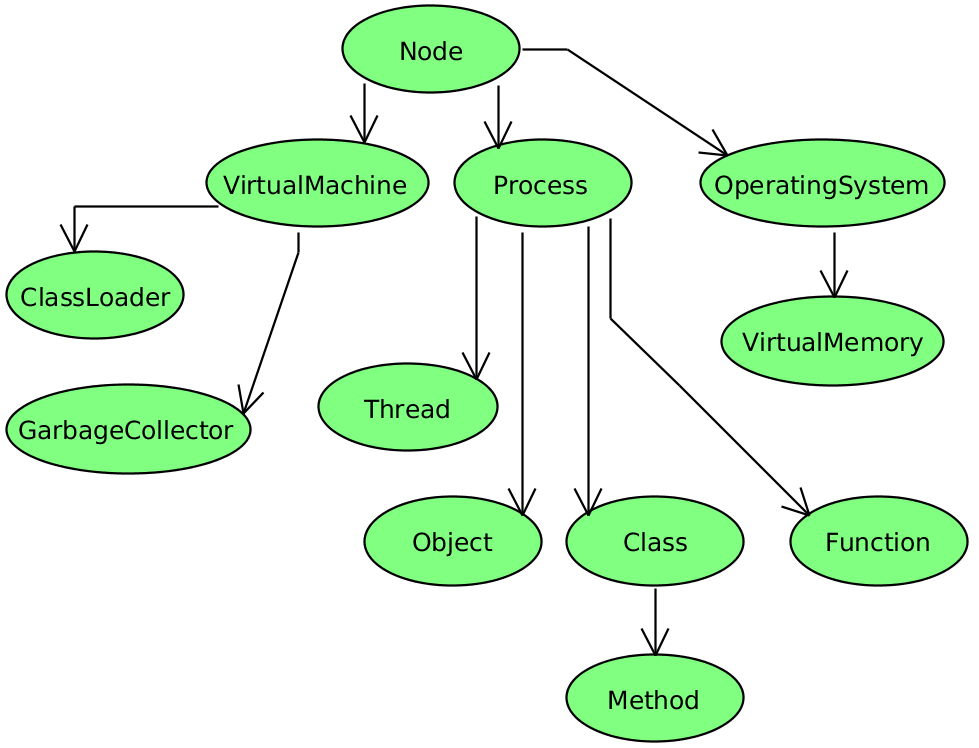
\includegraphics[width=0.7\textwidth]{onto_resources_has_a_software}
  \caption{Diagram of has-a relationship between software resources}
  \label{fig:onto_resources_has_a_software}
\end{figure}

\pagebreak

\subsection{Capabilities ontology}
\label{subsec:arch_knowledge_capabilitie}

For concepts related to capabilities of resources, only is-a relationships exists, which can be seen in
Figure~\ref{fig:onto_capabilities}. Because capability types are tightly coupled with resources, relations between them
reflects those between resources classes. 

There is one root concept, namely ResourceCapability, which subclasses rdf:Thing. It has 4 direct subtypes:
HardwareCapability, MemoryCapability, NodeCapability and SoftwareCapability. For hardware capability, there are only 2
deriving classes StorageCapability and CpuCapability. Since concept of VirtualMemory and PhysicalMemory are semantically
close, there is no need to subclass generic MemoryCapability, thus this type doesn't have any subtypes. NodeCapability
is another direct subtype of most generic ResourceCapability, which doesn't require any additional child types. 

Complex structure of software resources influences relationships between capabilities related to those components.
SoftwareCapability has 3 subtypes: OperatingSystemCapability, ProcessCapability and SoftwareComponentCapability.
Additionally, VirtualMachineCapability was extracted from ProcessCapability, because of same reasons that motivates
extraction of VirtualMachine resource type from Process - different semantics. The only one type that extends
SoftwareComponentCapability is ThreadCapability.


\begin{figure}[ht]
  \centering
  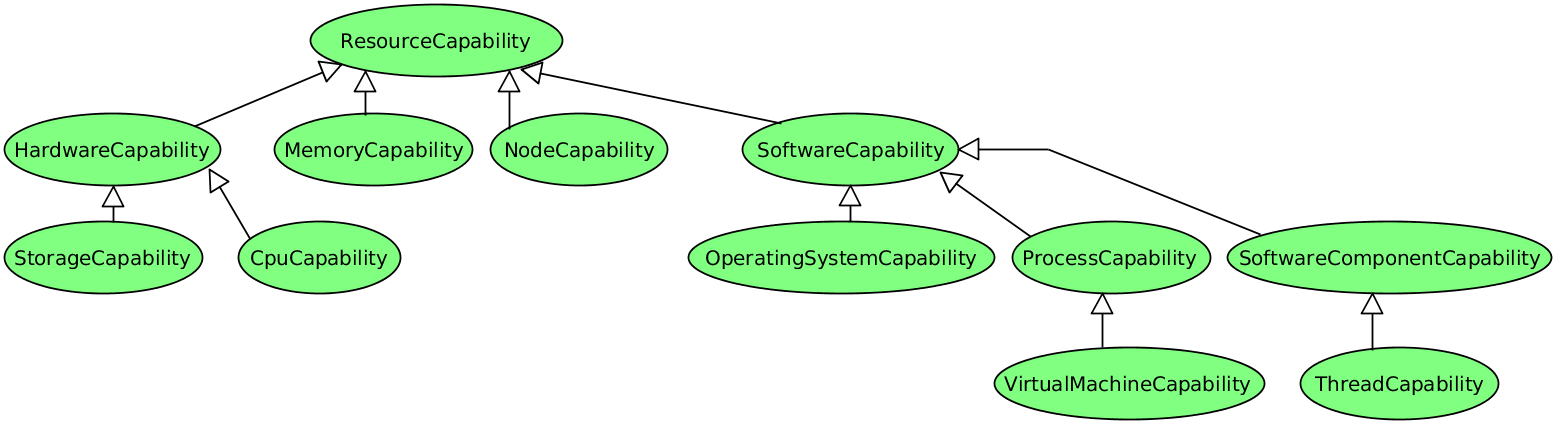
\includegraphics[width=1.0\textwidth]{onto_capabilities}
  \caption{Diagram of is-a relationship between capabilities}
  \label{fig:onto_capabilities}
\end{figure}







 
%---------------------------------------------------------------------------
% Transport proxy copmonent + it's realisations.
%
%---------------------------------------------------------------------------


\section{Transport Proxy component}
\label{sec:arch_tproxy}
 
Transport proxies are components responsible for communicating with external components that performs actual, low-level
analysis of processing tree and measurements. Each proxy implementation can specialize generic, ontology base concept
into item specific to platform or measuring system. All transport proxies implementation are being used by Monitoring
Hub component, and distributed in form of library (Java JAR). 

Because all proxies has rather straight purpose, further decomposition of those components won't be provided. In
following subsection, author covers overall design principles of Two transport proxies provided with initial
implementation of SemSimMon system.

 
\subsection{JMX Transport Proxy}

Implementation of transport proxy component responsible for integration with Java JMX consist of one root component -
JmxTransportProxy, several DiscoveryAgent and CapabilityProbe components. JmxTransportProxy component implements
interface used by other high-level system modules and performs all operations, delegating requests to appropriate
probes or discovery agents.

DiscoveryAgents are responsible for fetching all subresources of given resource. Each agent can be interpreted as a
mapping between ontology based, generic concept and item specific to JVM domain. Additionally, agents are responsible
for gathering all static properties of all discovered components.

If DiscoveryAgent can be seen as mapping between resource and JMX-specific entity, then CapabilityProbe should be
interpreted as mapping between generic capability described by ontology language into JMX specific feature. The only
responsibility of CapabilityProbe is to fetch value of capability that it can measure and using given resource.

To fulfill it's duties, JmxTransportProxy component maintains maps of discovery agents and capability probes. In both
cases map associates ontology URL of given concept to explicit probe or agent. Additionally it is responsible for
setting up and maintaining connection to JVM.


\subsection{OCM-G Transport Proxy}

OCM-G Transport Proxy component integrates SemSimMon with distributed monitoring system compliant with OMIS interface
specification. This implementation will use OMIS java bindings developed under OCM-G project. Design of this component
is similar to JMX transport proxy - there will be one OcmgTransportProxy component, responsible for maintaining
connections, associations and several probes and discovery agents.



